\SSCT{Les paramètres disponibles}{Parameters}

\SbSSCT{\'Epaisseur de ligne}{Line width}
\begin{center}
\RRR{15-3-1}
\end{center}

\begin{tabular}{|c|c|c|c|} \hline 
 \multicolumn{4}{|c|}{ \BS{tikz} \BS{draw}[line width=.2cm] (0,0) - - (1,1);}
 \\ \hline
\tikz \draw[line width=.2cm,blue] (0,0) - - (1,1) ;
 &  
\tikz \draw[ultra thin,blue] (0,0) - - (1,1) ;
 &  
\tikz \draw [very thin,blue] (0,0) - - (1,1) ;
 &  
\tikz \draw [thin,blue] (0,0) - - (1,1) ; 
 \\ \hline  
[\RDD{line width}=.2cm] & [\RDD{ultra thin}] & [\RDD{very thin}] & [\RDD{thin}] \\ 
  					& (0.1pt) & (0.2pt) & (0.4pt) \\ \hline
\tikz \draw[semithick,blue] (0,0) - - (1,1) ;
 &  
\tikz \draw[thick,blue] (0,0) - - (1,1) ;
 &  
\tikz \draw [very thick,blue] (0,0) - - (1,1) ;
 &  
\tikz \draw [ultra thick,blue] (0,0) - - (1,1) ; 
 \\ \hline  
[\RDD{semithick}] & [\RDD{thick}] & [\RDD{very thick}] & [\RDD{ultra thick}] \\
  (0.6pt)	& (0.8pt) & (1.2pt) & (1.6pt) \\ \hline 
\end{tabular} 

\SbSSCT{Dimensions disponibles}{Dimensions available}

\begin{tabular}{|c|c|} \hline  
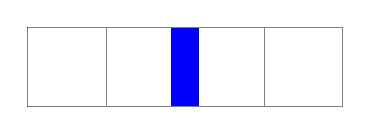
\begin{tikzpicture}[blue,line width=2pt,fill=green,baseline=.5cm]
\draw[use as bounding box][line width=0pt] (0,0)rectangle (4,1) ;
\draw[help lines] (0,0) grid (4,1); 
\draw[line width=10pt]  (2,0) to (2,1); 
  \end{tikzpicture}
& 
\BS{draw}[line width=10pt]  (2,0) to (2,1);  
\\ \hline 
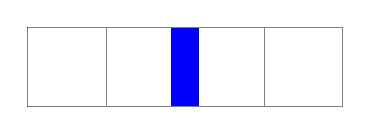
\begin{tikzpicture}[blue,line width=2pt,fill=green,baseline=.5cm]
\draw[use as bounding box][line width=0pt] (0,0)rectangle (4,1) ;
\draw[help lines] (0,0) grid (4,1); 
\draw[line width=10bp]  (2,0) to (2,1); 
  \end{tikzpicture}  
&  
\BS{draw}[line width=10bp]  (2,0) to (2,1); 
\\ \hline  
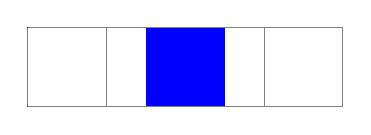
\begin{tikzpicture}[blue,line width=2pt,fill=green,baseline=.5cm]
\draw[use as bounding box][line width=0pt] (0,0)rectangle (4,1) ;
\draw[help lines] (0,0) grid (4,1); 
\draw[line width=10mm]  (2,0) to (2,1); 
  \end{tikzpicture}
&  
\BS{draw}[line width=10mm]  (2,0) to (2,1);
\\ \hline  
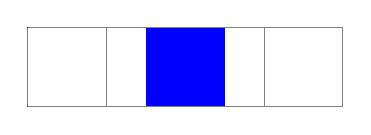
\begin{tikzpicture}[blue,line width=2pt,fill=green,baseline=.5cm]
\draw[use as bounding box][line width=0pt] (0,0)rectangle (4,1) ;
\draw[help lines] (0,0) grid (4,1); 
\draw[line width=1cm]  (2,0) to (2,1); 
  \end{tikzpicture}
&  
\BS{draw}[line width=1cm]  (2,0) to (2,1);
\\ \hline  
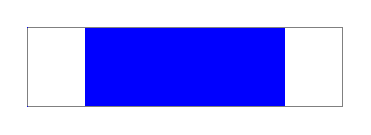
\begin{tikzpicture}[blue,line width=2pt,fill=green,baseline=.5cm]
\draw[use as bounding box][line width=0pt] (0,0) rectangle (4,1) ;
\draw[help lines] (0,0) grid (4,1); 
\draw[line width=1in]  (2,0) to (2,1); 
\end{tikzpicture}
&  
\BS{draw}[line width=1in]  (2,0) to (2,1);
\\ \hline
\end{tabular} 

\bigskip


\begin{tabular}{|c|c|} \hline  
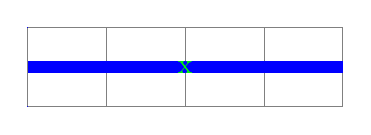
\begin{tikzpicture}[blue,line width=2pt,fill=green,baseline=.5cm]
\draw[use as bounding box][line width=0pt] (0,0) rectangle (4,1) ;
\draw[help lines] (0,0) grid (4,1); 
\draw[line width=1ex]  (0,0.5) to (4,.5);
\draw[green] (2,.5) node  {x};
\end{tikzpicture}
&  
\BS{draw}[line width=1ex]  (0,0.5) to (4,.5);
\\ \hline
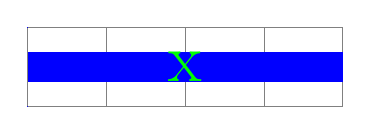
\begin{tikzpicture}[blue,line width=2pt,fill=green,baseline=.5cm]
\draw[use as bounding box][line width=0pt] (0,0) rectangle (4,1) ;
\draw[help lines] (0,0) grid (4,1); 
\Huge \draw[line width=1ex] (0,0.5) to (4,.5);
\draw[green] (2,.5) node  {x};
\end{tikzpicture}
&  
\BS{Huge} \BS{draw}[line width=1ex]  (0,0.5) to (4,.5);
\\ \hline
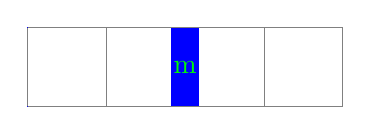
\begin{tikzpicture}[blue,line width=2pt,fill=green,baseline=.5cm]
\draw[use as bounding box][line width=0pt] (0,0) rectangle (4,1) ;
\draw[help lines] (0,0) grid (4,1); 
 \draw[line width=1em]  (2,0) to (2,1);
\draw[green] (2,.5) node  {m};
\end{tikzpicture}
&  
\BS{draw}[line width=1em]  (2,0) to (2,1);
\\ \hline
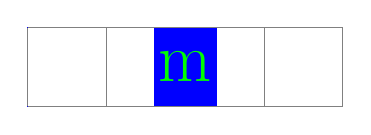
\begin{tikzpicture}[blue,line width=2pt,fill=green,baseline=.5cm]
\draw[use as bounding box][line width=0pt] (0,0) rectangle (4,1) ;
\draw[help lines] (0,0) grid (4,1); 
\Huge \draw[line width=1em]  (2,0) to (2,1);
\draw[green] (2,.5) node  {m};
\end{tikzpicture}
&  
\BS{Huge} \BS{draw}[line width=1em]  (2,0) to (2,1);
\\ \hline
\end{tabular} 


\SbSSCT{Terminaisons de lignes}{Terminators}

\begin{tabular}{|c|c|c|} \hline  
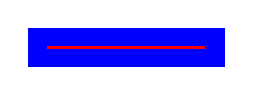
\begin{tikzpicture}[blue,line width=.5cm] 
\draw[line cap=rect]  (0,0) - - (2,0);
\draw[red,line width=1pt](0,0) - - (2,0);
\end{tikzpicture}
&
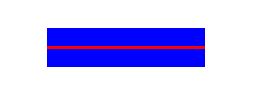
\begin{tikzpicture}[blue,line width=.5cm] 
\draw[line cap=butt]  (0,0) - - (2,0);
\draw[red,line width=1pt](0,0) - - (2,0);
\end{tikzpicture}  
&
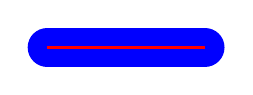
\begin{tikzpicture}[blue,line width=.5cm] 
\draw[line cap=round]  (0,0) - - (2,0);
\draw[red,line width=1pt](0,0) - - (2,0);
\end{tikzpicture}  \\ 
\hline [\RDD{line cap}=\RDDX{rect}{line cap}] & [\RDD{line cap}=\RDDX{butt}{line cap}] &  
[\RDD{line cap}=\RDDX{round}{line cap}]\\ 
\hline 
\end{tabular} 


\SbSSCT{Jonction de lignes}{Lines junction}


\begin{tabular}{|c|c|c|} \hline 

 \multicolumn{3}{|c|}{ \BS{draw}[\RDD{line join}=\RDDX{round}{line join}] (0,0)  - - (2,1) - - (0,2);}
 \\ \hline
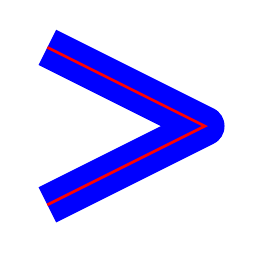
\begin{tikzpicture}[blue,line width=.5cm] 
\draw[line join=round] (0,0)  -- (2,1) -- (0,2);
\draw[red,line width=1pt](0,0)  -- (2,1) -- (0,2);
\end{tikzpicture}
& 
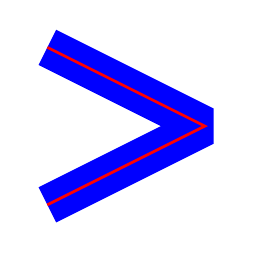
\begin{tikzpicture}[,blue,line width=.5cm] 
\draw[line join=bevel] (0,0)  -- (2,1) -- (0,2);
\draw[red,line width=1pt](0,0)  -- (2,1) -- (0,2);
\end{tikzpicture}
&
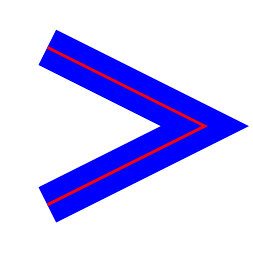
\begin{tikzpicture}[blue,line width=.5cm]  
\draw[line join=miter] (0,0)  -- (2,1) -- (0,2);
\draw[red,line width=1pt](0,0)  -- (2,1) -- (0,2);
\end{tikzpicture}
\\ \hline  
[\RDD{line join}=\RDDX{round}{line join}] &  
[\RDD{line join}=\RDDX{bevel}{line join}] &  
[\RDD{line join}=\RDDX{miter}{line join}] 
\\ \hline 
\end{tabular} 
\bigskip

\begin{tabular}{|c|c|c|} \hline 
 \multicolumn{3}{|c|}{  \BS{draw}[\RDD{miter limit}=1]  (0,0) - - (2,1) - - (0,2);} \\
\multicolumn{3}{|c|}{   (\dft{} : miter limit=10) }
 \\ \hline 
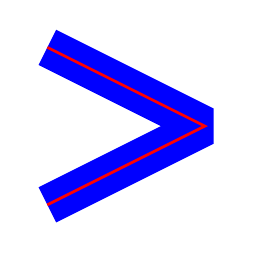
\begin{tikzpicture}[blue,line width=.5cm] 
\draw[miter limit=1]  (0,0) -- (2,1) -- (0,2);
\draw[red,line width=1pt](0,0)  -- (2,1) -- (0,2);
\end{tikzpicture}
&  
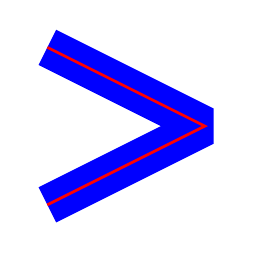
\begin{tikzpicture}[blue,line width=.5cm] 
\draw[miter limit=2]  (0,0) -- (2,1) -- (0,2);
\draw[red,line width=1pt](0,0)  -- (2,1) -- (0,2);
\end{tikzpicture}
&  
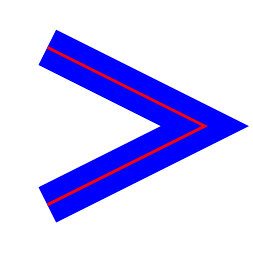
\begin{tikzpicture}[blue,line width=.5cm] 
\draw[miter limit=3]  (0,0) -- (2,1) -- (0,2);
\draw[red,line width=1pt](0,0)  -- (2,1) -- (0,2);
\end{tikzpicture}
\\ \hline miter limit=1 & miter limit=2 & miter limit=3 \\ 
\hline 
\end{tabular} 

\SbSSCT{Styles de ligne}{Line styles}

\begin{center}
\RRR{15-3-2}
\end{center}

\begin{tabular}{|c|c|c|c|} \hline 
 \multicolumn{3}{|c|}{ \BS{tikz} \BS{draw}[\RDD{solid},line width=2mm] (0,0) - - (2,1);}
 \\ \hline
\tikz \draw[solid,line width=2mm,blue] (0,0) - - (2,1) ;
& &
 \\ \hline
 [\RDD{solid}] & &
\\ \hline 
   
\tikz \draw[dotted,line width=2mm,blue] (0,0) - - (2,1) ;
 &  
\tikz \draw [densely dotted,line width=2mm,blue] (0,0) - - (2,1) ;
 &  
\tikz \draw [loosely dotted,line width=2mm,blue] (0,0) - - (2,1) ;
 \\ \hline  
 [\RDD{dotted}] & [\RDD{densely dotted}] & [\RDD{loosely dotted}] 
\\ 	\hline

\tikz \draw[dashed,line width=2mm,blue] (0,0) - - (2,1) ;
 &  
\tikz \draw[densely dashed,line width=2mm,blue] (0,0) - - (2,1) ;
 &  
\tikz \draw [loosely dashed,line width=2mm,blue] (0,0) - - (2,1) ;
\\ 	\hline
[\RDD{dashed}] & [\RDD{densely dashed}] & [\RDD{loosely dashed}]
\\ \hline 
\tikz \draw [dash dot,line width=2mm,blue] (0,0) - - (2,1) ;
&
\tikz \draw [densely dash dot,line width=2mm,blue] (0,0) - - (2,1) ;
&
\tikz \draw [loosely dash dot,line width=2mm,blue] (0,0) - - (2,1) ;
\\ \hline  
[\RDD{dash dot}] & [\RDD{densely dash dot}] & [\RDD{loosely dash dot}] 
\\ \hline 
\tikz \draw [dash dot dot,line width=2mm,blue] (0,0) - - (2,1) ;
&
\tikz \draw [densely dash dot dot,line width=2mm,blue] (0,0) - - (2,1) ;
&
\tikz \draw [loosely dash dot dot,line width=2mm,blue] (0,0) - - (2,1) ;
\\ \hline  
[\RDD{dash dot dot}] & [\RDD{densely dash dot dot}] & [\RDD{loosely dash dot dot}]
\\ \hline
\end{tabular}

\bigskip
\begin{tabular}{|c|c|} \hline  
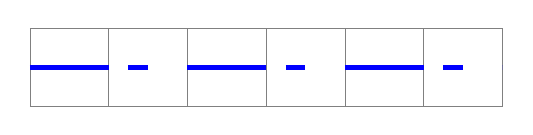
\begin{tikzpicture}[blue,line width=2pt,fill=green,baseline=.5cm]
\draw[help lines] (0,0) grid (6,1); 
\draw[dash pattern=on 1cm off .25cm on .25cm off .5cm,ultra thick,blue] (0,0.5) - - (6,.5) ; 
  \end{tikzpicture}
\\ \hline 
[\RDD{dash pattern}= \BDD{on} 1cm \BDD{off} 0.25cm \BDD{on} 0.25cm \BDD{off} 0.5cm] 
\\ \hline
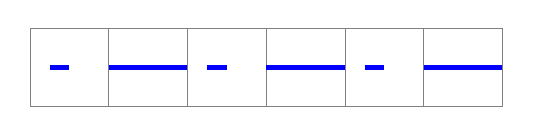
\begin{tikzpicture}[blue,line width=2pt,fill=green,baseline=.5cm]
\draw[help lines] (0,0) grid (6,1); 

\draw[dash pattern=on 1cm off .25cm on .25cm off .5cm,dash phase=1cm,ultra thick,blue] (0,0.5) - - (6,.5) ;
  \end{tikzpicture}
\\ \hline  

[dash pattern=on 1cm off .25cm on .25cm off .5cm,\RDD{dash phase}=1cm] 
\\ \hline 
\end{tabular}

\bigskip

\begin{center}
\RRR{15-3-4}
\end{center}


\begin{tabular}{|c|c|c|c|} \hline 
 \multicolumn{4}{|c|}{ \BS{tikz} \BS{draw}[line width=.2cm,\RDD{double}] (0,0) - - (1,1);}
 \\ \hline

\tikz \draw[line width=.2cm,double,blue] (0,0) - - (1,1) ;
&
\tikz \draw[line width=.2cm,draw=blue,double=red] (0,0) - - (1,1) ;
&
\tikz \draw[line width=.2cm,double distance=.3cm] (0,0) - - (1,1) ;
&
\tikz \draw[line width=.2cm,double,double distance between line centers=.3cm] (0,0) - - (1,1) ;
\\ \hline 
\RDD{double} & draw=blue,double=red & \RDD{double distance}=.3cm & \RDD{double distance between line centers} \\
& & &  =.3cm
\\ \hline 
\end{tabular}

\bigskip


\begin{tabular}{|c|c|} \hline  
 \multicolumn{2}{|c|}{ \BS{Huge} = \BS{tikz} \BS{draw}[\RDD{double equal sign distance}] (0,0) - - (4,0);}
 \\ \hline
 \rule[-.3cm]{0pt}{1cm}
{\Huge  = \tikz[baseline=-.2cm] \draw[blue,double equal sign distance] (0,0) - - (4,0) ;}
&  
{\large  = \tikz[baseline=-.1cm]  \draw[blue,double equal sign distance] (0,0) - - (4,0) ;}
\\ \hline  
\BS{Huge}
&  
\BS{large}
\\ \hline 
\end{tabular} 

\SbSSCT{Remplissage en motifs}{Fillings}
\label{lib-patterns}

\begin{center}
\RRR{15-5-1} \RRR{60}
\end{center}

\maboite{\BS{usetikzlibrary}\AC{patterns}}
 

\begin{tabular}{|c|c|c|} \hline  
 \multicolumn{3}{|c|}{ \BS{draw}[\RDD{pattern}= \RDDX{dots}{pattern}] (0,0) - - (3,1);}
 \\ \hline

\begin{tikzpicture}
\draw[white] (0,0)--(0,1.2);
\draw[pattern=dots] (0,0) rectangle (3,1);
\end{tikzpicture}
&  
\begin{tikzpicture}
\draw[pattern=fivepointed stars] (0,0) rectangle (3,1);
\end{tikzpicture}
&  
\begin{tikzpicture}
\draw[pattern=sixpointed stars] (0,0) rectangle (3,1);
\end{tikzpicture}
\\ \hline  
\RDDX{dots}{pattern} & \RDDX{fivepointed stars}{pattern} & \RDDX{sixpointed stars}{pattern}   
\\ \hline

\begin{tikzpicture}
\draw[white] (0,0)--(0,1.2);
\draw[pattern=grid] (0,0) rectangle (3,1);
\end{tikzpicture}
&
\begin{tikzpicture}
\draw[pattern=horizontal lines] (0,0) rectangle (3,1);
\end{tikzpicture}
&  
\begin{tikzpicture}
\draw[pattern=vertical lines] (0,0) rectangle (3,1);
\end{tikzpicture}
\\ \hline  
\RDDX{grid}{pattern} & \RDDX{horizontal lines}{pattern} & \RDDX{vertical lines}{pattern} 
\\ \hline  

\begin{tikzpicture}
\draw[white] (0,0)--(0,1.2);
\draw[pattern=north east lines] (0,0) rectangle (3,1);
\end{tikzpicture}
&  
\begin{tikzpicture}
\draw[pattern=north west lines] (0,0) rectangle (3,1);
\end{tikzpicture}
&
\begin{tikzpicture}
\draw[pattern=crosshatch] (0,0) rectangle (3,1);
\end{tikzpicture}

\\ \hline
 \RDDX{north east lines}{pattern} & 
 \RDDX{north west lines}{pattern}  &  \RDDX{rosshatch}{pattern}
\\ \hline

 
\begin{tikzpicture}
\draw[white] (0,0)--(0,1.2);
\draw[pattern=crosshatch dots] (0,0) rectangle (3,1);
\end{tikzpicture}
&  
\begin{tikzpicture}
\draw[pattern=bricks] (0,0) rectangle (3,1);
\end{tikzpicture}
& 
\begin{tikzpicture}
\draw[pattern=checkerboard] (0,0) rectangle (3,1);
\end{tikzpicture}
 
\\ \hline
\RDDX{crosshatch dots}{pattern}  & \RDDX{bricks}{pattern} & \RDDX{checkerboard}{pattern}
\\ \hline
\end{tabular} 

\bigskip

\begin{tabular}{|c|} \hline  
\begin{tikzpicture}
\draw[pattern=fivepointed stars,pattern color=red] (0,0) rectangle (3,1);
\end{tikzpicture}
\\ \hline  
\BS{draw}[pattern=fivepointed stars,\RDD{pattern color}=red] (0,0) rectangle (3,1);
\\ \hline 
\end{tabular}

\bigskip

\begin{tabular}{|c|c|c|} \hline  
 \multicolumn{3}{|c|}{ \BS{draw}[pattern=\RDDX{checkerboard light gray}{pattern}] (0,0) - - ((3,2) ;}
 \\ \hline
\begin{tikzpicture}
\draw[pattern=checkerboard light gray] (0,0) rectangle (3,1);
\end{tikzpicture}
&
\begin{tikzpicture}
\draw[pattern=horizontal lines light gray] (0,0) rectangle (3,1);
\end{tikzpicture}
&
\begin{tikzpicture}
\draw[pattern=horizontal lines gray] (0,0) rectangle (3,1);
\end{tikzpicture} 
 \\ \hline
\RDDX{checkerboard light gray}{pattern} &  \RDDX{horizontal lines light gray}{pattern} & \RDDX{horizontal lines gray}{pattern}
 \\ \hline
\begin{tikzpicture}
\draw[pattern=horizontal lines dark gray] (0,0) rectangle (3,1);
\end{tikzpicture}
&
\begin{tikzpicture}
\draw[pattern=horizontal lines light blue] (0,0) rectangle (3,1);
\end{tikzpicture}
&
\begin{tikzpicture}
\draw[pattern=horizontal lines dark blue] (0,0) rectangle (3,1);
\end{tikzpicture}
 \\ \hline
\RDDX{horizontal lines dark gray}{pattern} &  \RDDX{horizontal lines light blue}{pattern} & \RDDX{horizontal lines dark blue}{pattern}
 \\ \hline
 \begin{tikzpicture}
 \draw[pattern=crosshatch dots gray] (0,0) rectangle (3,1);
 \end{tikzpicture}
 &
 \begin{tikzpicture}
 \draw[pattern=crosshatch dots light steel blue] (0,0) rectangle (3,1);
 \end{tikzpicture}
 &
  \\ \hline
\RDDX{crosshatch dots gray}{pattern} & \RDDX{crosshatch dots light steel blue}{pattern}
&  \\ \hline
\end{tabular} 

\SbSSCT{Règle de remplissage}{Filling rule}

\begin{center}
\RRR{15-5-2}
\end{center}


\begin{tabular}{|c|c|} \hline 
\multicolumn{2}{|c|}{ nonzero rule (\dft{}) }
\\ \hline 
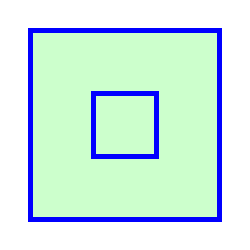
\begin{tikzpicture}[scale=.8,blue,baseline=0pt,line width=2pt]
\filldraw[fill=green!20] (0,0) -- (0,3) -- (3,3) -- (3,0) -- cycle  (1,1) -- (1,2) -- (2,2) --(2,1) -- cycle; 
\end{tikzpicture}
&  
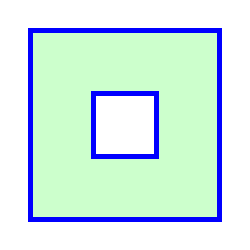
\begin{tikzpicture}[scale=.8,blue,baseline=0pt,line width=2pt]
\filldraw[fill=green!20] (0,0) -- (0,3) -- (3,3) -- (3,0) -- cycle  (1,1) -- (2,1) -- (2,2) --(1,2) -- cycle; 
\end{tikzpicture}
\\ \hline 
\BS{filldraw} [fill=green!20]  & \BS{filldraw} [fill=green!20] \\
(0,0) - - (0,3) - - (3,3) - - (3,0) - - cycle  &
(0,0) - - (0,3) - - (3,3) - - (3,0) - - cycle \\
(1,1) - - {\color{red}(1,2) - - (2,2) - -(2,1)} - - cycle ;  & 
(1,1) - - {\color{red}(2,1) - - (2,2) - -(1,2)} - - cycle; 
\\ \hline 
\end{tabular}


\begin{tabular}{|c|c||c|c|} \hline
\multicolumn{2}{|c|}{ even odd rule }
\\ \hline   
 \multicolumn{2}{|c||}{\BS[fill=[green] (0,0) - - (2,1) - - (1,2) circle (.5cm); } & 
  \multicolumn{2}{|c|}{\BS{filldraw}[fill=green] (0,0) -- (2,1) - - (1,2) circle (.5cm); }
 \\ \hline

\begin{tikzpicture}
\fill[green] (0,0) -- (2,1) -- (1,2) circle (.5cm);
\end{tikzpicture}
&  

\begin{tikzpicture}
\fill[even odd rule,green]  (0,0) -- (2,1) -- (1,2) circle (.5cm);
\end{tikzpicture}
&
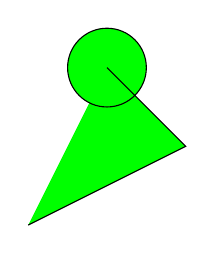
\begin{tikzpicture}
\filldraw[fill=green] (0,0) -- (2,1) -- (1,2) circle (.5cm);
\end{tikzpicture}
&  
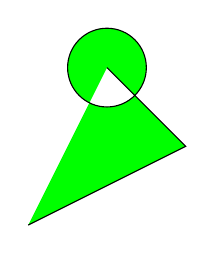
\begin{tikzpicture}
\filldraw[even odd rule,fill=green]  (0,0) -- (2,1) -- (1,2) circle (.5cm);
\end{tikzpicture}
\\ \hline 
[fill=green] & [\RDD{even odd rule},fill=green]  & [fill=green] & [\RDD{even odd rule},fill=green]
\\ \hline 
\end{tabular}

\SbSSCT{Remplissage à l'aide d'une image}{Filling with an image  }

\begin{center}
\RRR{15-6}
\end{center}


\begin{tabular}{|c|c|c|} \hline 
 \multicolumn{3}{|c|}{\BS{draw} [\RDD{path picture}=\{  \BS{node} at (path picture bounding box.center) }\\
 \multicolumn{3}{|c|}{ \AC{\BS{includegraphics}[height=3cm]\AC{tiger}\};}] (0,1) circle (1);}
\\   \hline 
\begin{tikzpicture}
\draw [path picture={
\node at (path picture bounding box.center){\includegraphics[height=3cm]{tiger}};}] (0,1) circle (1);
\end{tikzpicture}
&
\begin{tikzpicture}
\draw [path picture={
\node at (path picture bounding box.center){\includegraphics[height=3cm]{tiger}};}] (0,0) -- (-1,1) -- (0,2) -- (1,1) -- cycle;
\end{tikzpicture}
&
\begin{tikzpicture}
\draw [path picture={
\node at (path picture bounding box.center){\includegraphics[height=3cm]{tiger}};}] (1,0) parabola[parabola height=2cm] (3,0);
\end{tikzpicture}
\\ \hline 
(0,1) circle (1) & (0,0) - - (-1,1) - - (0,2) - - (1,1) - - cycle &  (1,0) parabola[parabola height=2cm] (3,0)\\ 
\hline
\end{tabular} 
\bigskip

\begin{tabular}{|c|c|c|c|c|} \hline 
 \multicolumn{5}{|c|}{\BS{draw} [path picture=\{  \BS{node} at (\RDD{path picture bounding box}.north) }\\
 \multicolumn{5}{|c|}{ \AC{\BS{includegraphics}[height=3cm]\AC{tiger}\};}] (0,1) circle (1);}
\\   \hline 
\begin{tikzpicture}
\draw [path picture={
\node at (path picture bounding box.north){\includegraphics[height=3cm]{tiger}};}] (0,1) circle (1);
\end{tikzpicture}
&
\begin{tikzpicture}
\draw [path picture={
\node at (path picture bounding box.south){\includegraphics[height=3cm]{tiger}};}] (0,1) circle (1);
\end{tikzpicture}
&
\begin{tikzpicture}
\draw [path picture={
\node at (path picture bounding box.east){\includegraphics[height=3cm]{tiger}};}] (0,1) circle (1);
\end{tikzpicture}
&
\begin{tikzpicture}
\draw [path picture={
\node at (path picture bounding box.west){\includegraphics[height=3cm]{tiger}};}] (0,1) circle (1);
\end{tikzpicture}
&
\begin{tikzpicture}
\draw [path picture={
\node at (path picture bounding box.south east){\includegraphics[height=3cm]{tiger}};}] (0,1) circle (1);
\end{tikzpicture}
\\   \hline 
north & south & east & west &south east
\\   \hline 
\end{tabular} 

\SbSSCT{Ombrage}{Shading}


\SbSbSSCT{Ombrages disponibles}{Shadings available}
\begin{center}
\RRR{15-7}
\end{center}

\begin{tabular}{|c|c|} \hline  
\begin{tikzpicture}
\draw[white] (0,0)--(0,1.2);
\shade (0,0) rectangle (3,1);
\end{tikzpicture}
&  
\begin{tikzpicture}
\shadedraw (0,0) rectangle (3,1);
\end{tikzpicture}
\\ \hline  
\BSS{shade} (0,0) rectangle (3,1); & \BSS{shadedraw} (0,0) rectangle (3,1);\\ 
\hline 
\end{tabular} 

\bigskip

\begin{tabular}{|c|c|c|} \hline 
 \multicolumn{3}{|c|}{\BS{shadedraw}[\RDD{shading}=\RDDX{axis}{shading}](0,0) rectangle (3,1); }
 \\ \hline
 
\begin{tikzpicture}
\draw[white] (0,0)--(0,1.2);
\shadedraw[shading=axis] (0,0) rectangle (3,1);
\end{tikzpicture}
&  
\begin{tikzpicture}
\shadedraw[shading=radial] (0,0) rectangle (3,1);
\end{tikzpicture}
&  
\begin{tikzpicture}
\shadedraw[shading=ball] (0,0) rectangle (3,1);
\end{tikzpicture}

\\ \hline  
\RDDX{axis}{shading}  & \RDDX{radial}{shading}  & \RDDX{ball}{shading}\\ 
\hline 
\end{tabular} 

\bigskip

\begin{tabular}{|c|c|c|} \hline  
\begin{tikzpicture}
\draw[white] (0,0)--(0,1.2);
\shadedraw[left color=red] (0,0) rectangle (3,1);
\end{tikzpicture}
&  
\begin{tikzpicture}
\shadedraw[right color=green] (0,0) rectangle (3,1);
\end{tikzpicture}
&  
\begin{tikzpicture}
\shadedraw[left color=red,right color=green] (0,0) rectangle (3,1);
\end{tikzpicture}
\\ \hline  
[\RDD{left color}=red] & [\RDD{right color}=green]  &  \RDD{left color}=red,\RDD{right color}=green \\ 
\hline 
\begin{tikzpicture}
\draw[white] (0,0)--(0,1.2);
\shadedraw[top color=red] (0,0) rectangle (3,1);
\end{tikzpicture}
&  
\begin{tikzpicture}
\shadedraw[bottom color=green] (0,0) rectangle (3,1);
\end{tikzpicture}
&  
\begin{tikzpicture}
\shadedraw[middle color=red] (0,0) rectangle (3,1);
\end{tikzpicture}
\\ \hline  
[\RDD{top color}=red] & [\RDD{bottom color}=green]  &  \RDD{middle color}=red \\ 
\hline 

\end{tabular} 

\bigskip

\begin{tabular}{|c|c|c|} \hline  
\begin{tikzpicture}
\draw[white] (0,0)--(0,1.2);
\shadedraw[shading angle=90] (0,0) rectangle (3,1);
\end{tikzpicture}
&  
\begin{tikzpicture}
\shadedraw[right color=green,shading angle=45] (0,0) rectangle (3,1);
\end{tikzpicture}
&  
\begin{tikzpicture}
\shadedraw[left color=red,shading angle=-45] (0,0) rectangle (3,1);
\end{tikzpicture}

\\ \hline  
 & \RDD{right color}=green  & left color=red \\ 
\RDD{shading angle}=90 & [\RDD{shading angle}=45]  & \RDD{shading angle}=-45 \\
\hline 
\end{tabular} 

\bigskip

\begin{tabular}{|c|c|c|} \hline  
\begin{tikzpicture}
\draw[white] (0,0)--(0,1.2);
\shadedraw[inner color=red] (0,0) rectangle (3,1);
\end{tikzpicture}
&  
\begin{tikzpicture}
\shadedraw[outer color=green] (0,0) rectangle (3,1);
\end{tikzpicture}
&  
\begin{tikzpicture}
\shadedraw[outer color=green,inner color=red] (0,0) rectangle (3,1);
\end{tikzpicture}

\\ \hline  
 \RDD{inner color}=red & \RDD{outer color}=green  & \RDD{inner color}=red \RDD{outer color}=green
 \\ \hline 
\end{tabular}

\newpage
\SbSbSSCT{Bibliothèque shadings}{Shading library}
\begin{center}
 \RRR{65}
\end{center}
 
 \maboite{\BS{usetikzlibrary}\AC{shadings}}
\label{lib-shadings}

\begin{tabular}{|c|c|c|c|c|} \hline
 \multicolumn{5}{|c|}{\BS{shadedraw}[\RDD{upper left}=red] (0,0) rectangle (2,2) ; }
 \\ \hline 
\begin{tikzpicture}
\shadedraw[upper left=red] (0,0) rectangle (2,2);
\end{tikzpicture} 
&  
\begin{tikzpicture}
\shadedraw[upper right=green] (0,0) rectangle (2,2);
\end{tikzpicture} 
&  
\begin{tikzpicture}
\shadedraw[lower left=blue] (0,0) rectangle (2,2);
\end{tikzpicture} 
&  
\begin{tikzpicture}
\shadedraw[lower right=yellow] (0,0) rectangle (2,2);
\end{tikzpicture} 
&
\begin{tikzpicture}
\shadedraw[upper left=red,upper right=green,
lower left=blue,lower right=yellow] (0,0) rectangle (2,2);
\end{tikzpicture} 
\\ \hline 
 \RDD{upper left}=red &  \RDD{upper right}=green &  \RDD{lower left}=blue  &  \RDD{lower right}=yellow & \\ 
\hline 
\end{tabular}  

\bigskip

\begin{tabular}{|c|c|c|} \hline 
 \multicolumn{3}{|c|}{\BS{shadedraw}[shading=\RDDX{color wheel}{shading}] (0,0) rectangle (2,2) ; }
 \\ \hline 
\begin{tikzpicture}
\shadedraw[shading=color wheel] (0,0) rectangle (2,2);
\end{tikzpicture} 
&
\begin{tikzpicture}
\shadedraw[shading=color wheel black center] (0,0) rectangle (2,2);
\end{tikzpicture}
&
\begin{tikzpicture}
\shadedraw[shading=color wheel white center] (0,0) rectangle (2,2);
\end{tikzpicture}
\\ \hline 
shading=\RDDX{color wheel}{shading} & shading=\RDDX{color wheel black center}{shading} & 
shading=\RDDX{color wheel white center}{shading}
\\ \hline 
\end{tabular} 

\bigskip

\begin{tabular}{|c|} \hline  
\begin{tikzpicture}
\shadedraw[shading=Mandelbrot set] (0,0) rectangle (2,2);
\end{tikzpicture}
\\\hline  
shading=\RDDX{Mandelbrot set}{shadingv}
\\ \hline 
\end{tabular} 



